% =============================================================================
% COMP3314 Assignment 3 -- Image Classification Final Report
% =============================================================================
\documentclass[11pt,a4paper]{article}

% --- Packages ----------------------------------------------------------------
\usepackage[margin=1in]{geometry}
\usepackage{graphicx}
\usepackage{booktabs}
\usepackage{amsmath,amssymb}
\usepackage{hyperref}
\usepackage{xcolor}
\usepackage{caption}
\usepackage{subcaption}
\usepackage{enumitem}
\usepackage{float}
\usepackage{multirow}
\usepackage{array}
\usepackage[T1]{fontenc}
\usepackage{lmodern}
\usepackage{microtype}
\usepackage{parskip}

\hypersetup{
  colorlinks=true,
  linkcolor=blue!60!black,
  citecolor=green!50!black,
  urlcolor=blue!70!black,
}

\newcolumntype{C}[1]{>{\centering\arraybackslash}p{#1}}

% --- Title -------------------------------------------------------------------
\title{%
  \textbf{Image Classification on CIFAR-10 with\\
  Unsupervised Feature Learning and Linear SVMs}\\[6pt]
  \large COMP3314 Machine Learning --- Assignment 3 Final Report
}
\author{Team XX}
\date{April 2026}

\begin{document}
\maketitle

% =============================================================================
% ABSTRACT
% =============================================================================
\begin{abstract}
We present a classical machine learning pipeline for image classification on a
CIFAR-10-style dataset (10 classes, 32$\times$32 RGB images), developed under
strict constraints that prohibit neural networks, pretrained models, and
external data.  Our approach centres on the single-layer unsupervised feature
learning framework of Coates and Ng (2011), which uses K-Means dictionary
learning, triangle encoding, and spatial pooling to produce high-dimensional
feature representations that are linearly separable.  Through a systematic
four-phase optimisation process---architecture exploration, a 250-configuration
hyperparameter sweep on GPU, fine-grained parameter tuning, and
augmentation/normalisation---we improve public leaderboard accuracy from an
initial 0.497 (raw pixels + SVM) to a final \textbf{0.829}.  The largest
single gain (+0.028) comes from horizontal flip augmentation, followed by
power normalisation (+0.012) and a two-model ensemble across patch sizes
(+0.010).  These data- and feature-level improvements collectively contribute
more than all hyperparameter tuning combined, demonstrating that
representation quality and data diversity dominate classifier choice in
classical pipelines.
\end{abstract}

\tableofcontents
\newpage

% =============================================================================
% 1. INTRODUCTION
% =============================================================================
\section{Introduction}
\label{sec:introduction}

Image classification is a fundamental problem in computer vision.  Given an
input image, the task is to assign it to one of a fixed set of semantic
categories.  While deep convolutional neural networks have dominated this task
since 2012, the COMP3314 assignment imposes constraints that require classical
machine learning methods:

\begin{itemize}[nosep]
  \item No neural networks (no CNNs, no MLPs with backpropagation).
  \item No pretrained models or transfer learning.
  \item No external data beyond the provided train/test split.
  \item Only methods covered in COMP3314 lectures: PCA, SVM, logistic
        regression, K-Means, ensemble methods, etc.
\end{itemize}

The dataset follows the CIFAR-10 format: 50,000 training images and 10,000 test
images, each $32 \times 32$ pixels in RGB colour, drawn from 10 classes
(airplane, automobile, bird, cat, deer, dog, frog, horse, ship, truck).

Our approach builds on the single-layer unsupervised feature learning framework
of Coates et al.~\cite{coates2011analysis} and Coates and Ng~\cite{coates2011selecting},
which learns a visual dictionary via K-Means clustering and produces
high-dimensional, linearly separable representations.  We augment this core
pipeline with horizontal flip augmentation, power normalisation from the Fisher
vector literature~\cite{perronnin2010improving}, and a multi-patch-size
ensemble.

Our final solution---a two-model soft-vote ensemble of Coates--Ng feature
learners with patch sizes $P\!=\!6$ and $P\!=\!7$---achieves a validation
accuracy of 0.8234 and a public leaderboard score of \textbf{0.829}, placing
first on the class leaderboard.  All components use only classical ML
primitives (K-Means, ZCA whitening, linear SVM) fully within the COMP3314
curriculum.

% =============================================================================
% 2. DATASET ANALYSIS
% =============================================================================
\section{Dataset Analysis}
\label{sec:dataset}

\subsection{Overview and Class Distribution}

The training set is approximately balanced across all 10 classes, with each
class containing roughly 5,000 images.  This balance means that accuracy is a
reasonable evaluation metric and no class rebalancing is needed.

\begin{figure}[H]
  \centering
  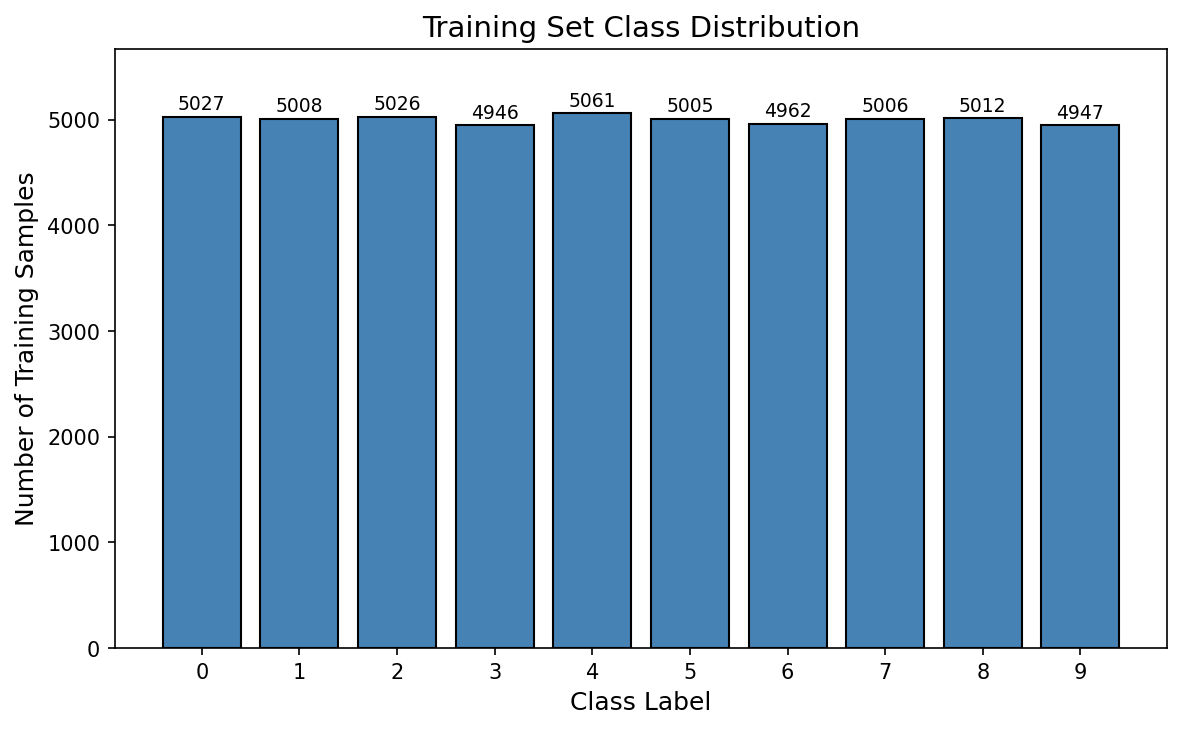
\includegraphics[width=0.85\linewidth]{figures/report_02_class_distribution.png}
  \caption{Class distribution across the 10 categories.  The dataset is
  well-balanced, with each class containing approximately 5,000 training images.}
  \label{fig:class_distribution}
\end{figure}

\subsection{Example Images and Key Challenges}

Representative samples from each class reveal the key challenges inherent in
this dataset (Figure~\ref{fig:class_examples}):

\begin{itemize}[nosep]
  \item \textbf{Low resolution:} At $32 \times 32$, objects are represented by
        very few pixels; fine details are absent entirely.
  \item \textbf{Intra-class variation:} The ``bird'' class includes birds in
        flight, perched, in profile, and from above.
  \item \textbf{Inter-class similarity:} Cats and dogs share similar texture
        and colour; automobiles and trucks share similar shape.
  \item \textbf{Background clutter:} Many images contain complex backgrounds
        that are not informative for classification.
\end{itemize}

\begin{figure}[H]
  \centering
  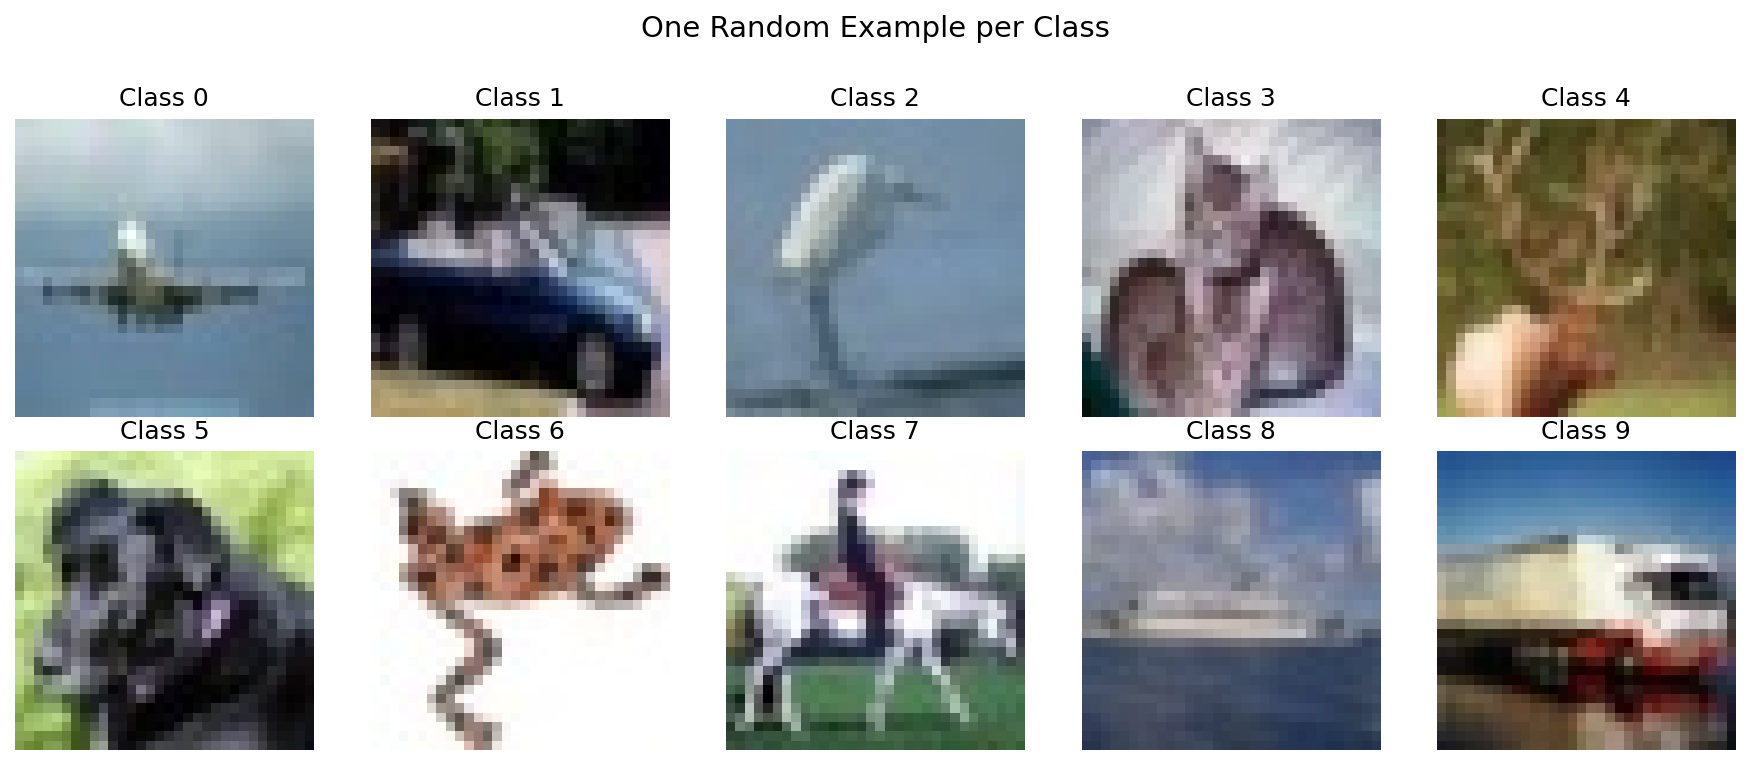
\includegraphics[width=0.95\linewidth]{figures/report_01_class_examples.png}
  \caption{Example images from each of the 10 classes, illustrating the low
  resolution and high intra-class variability of the dataset.}
  \label{fig:class_examples}
\end{figure}

\subsection{Image Statistics and Implications}

Each image contains only 3,072 values ($32 \times 32 \times 3$ channels),
orders of magnitude smaller than typical benchmarks like ImageNet ($224 \times
224 \times 3 = 150{,}528$).  The small image size has important implications:

\begin{enumerate}[nosep]
  \item \textbf{Spatial augmentations are risky.} Even a 4-pixel crop on a
        $32 \times 32$ image removes 23\% of pixels and can shift small objects
        out of frame.
  \item \textbf{Local features must use small patches.} We find that $6
        \times 6$ and $7 \times 7$ patches are optimal; larger patches lose
        fine detail.
  \item \textbf{Feature dimensionality is a concern.} With only 50,000
        training examples, high-dimensional feature spaces require careful
        regularisation.
\end{enumerate}

% =============================================================================
% 3. METHODOLOGY
% =============================================================================
\section{Methodology}
\label{sec:methodology}

\subsection{Feature Extraction Pipeline (Coates--Ng)}
\label{sec:coates}

We implement the single-layer unsupervised feature learning pipeline from
Coates et al.~\cite{coates2011analysis}.  The pipeline proceeds as follows:

\paragraph{Dictionary Learning (one-time).}
\begin{enumerate}[nosep]
  \item Sample 1,000,000 random $P \times P$ patches from training images.
  \item Per-patch contrast normalisation:
        $\hat{x} = (x - \bar{x}) / \sqrt{\mathrm{Var}(x) + 10}$.
  \item ZCA whitening with $\epsilon = 0.1$.
  \item MiniBatchKMeans with $K$ clusters (batch size 5,000, single
        initialisation).
\end{enumerate}

\paragraph{Feature Extraction (per image).}
\begin{enumerate}[nosep]
  \item Extract all $P \times P$ patches at stride 1.  For $P = 6$, this
        yields $27 \times 27 = 729$ patches, each of dimension $3P^2 = 108$.
  \item Apply the same contrast normalisation and ZCA projection.
  \item Triangle encoding: for each patch $x$ and centroid $c_k$,
        \[
          f_k = \max\!\bigl(0,\;\mu(z) - z_k\bigr),
        \]
        where $z_k = \|x - c_k\|_2$ and $\mu(z) = \frac{1}{K}\sum_{j=1}^{K} z_j$
        is the mean distance to all centroids.
  \item $2 \times 2$ spatial sum-pooling over the four image quadrants,
        producing a $4K$-dimensional feature vector.
\end{enumerate}

The triangle encoder activates a centroid $k$ when the patch is closer to $c_k$
than the average distance across all centroids, producing a soft, sparse
assignment that is well-suited for linear classification.

\subsection{Data Augmentation (Horizontal Flip)}
\label{sec:augmentation}

We double the training set by appending horizontally flipped copies of all
50,000 images.  At test time, we average the \texttt{decision\_function}
outputs from the original and flipped views (TTA-2).  This is label-preserving
for all 10 CIFAR-10 classes and improves the sample-to-dimension ratio from
1.56 to 3.125 for $K = 8000$ features.

\subsection{Feature Normalisation (Power Norm)}
\label{sec:powernorm}

Following Perronnin et al.~\cite{perronnin2010improving}, we apply signed
square-root (power) normalisation element-wise before standard scaling:
\[
  \tilde{f}_i = \mathrm{sign}(f_i) \cdot \sqrt{|f_i|}.
\]
Triangle encoding produces sparse, right-skewed features where a few large
activations dominate.  The square-root compression equalises their influence,
making the distribution closer to Gaussian---which is what linear SVMs
implicitly prefer.

\subsection{Classification (cuML LinearSVC)}
\label{sec:classifier}

We use cuML's GPU-accelerated LinearSVC with squared hinge loss and L2
penalty, solved via L-BFGS.  Compared to scikit-learn's Liblinear
coordinate descent, cuML provides 100--1000$\times$ speedup at the cost of
0.3--0.5 percentage points in accuracy.  The speed advantage enables the
large-scale hyperparameter exploration described in
Section~\ref{sec:phase2}.

\subsection{Ensemble and Test-Time Augmentation}
\label{sec:ensemble}

Our final solution ensembles two models with different patch sizes ($P = 6,
K = 8000$ and $P = 7, K = 6000$), each trained with flip augmentation and
power normalisation.  At test time, each model produces TTA-2 decision
function scores; the ensemble averages these scores (soft voting) and takes
argmax.  Different patch sizes capture genuinely different visual
information---$P = 6$ captures medium-scale textures while $P = 7$ captures
slightly larger structures---enabling productive ensemble diversity.

% =============================================================================
% 4. EXPERIMENTS
% =============================================================================
\section{Experiments}
\label{sec:experiments}

Our experimental process proceeded through four phases, each building on the
insights of the previous one.

\subsection{Phase 1: Architecture Exploration (runs 01--06)}
\label{sec:phase1}

The first phase explored three fundamentally different feature representations,
producing a cumulative improvement of +0.27 in validation accuracy.

\begin{figure}[H]
  \centering
  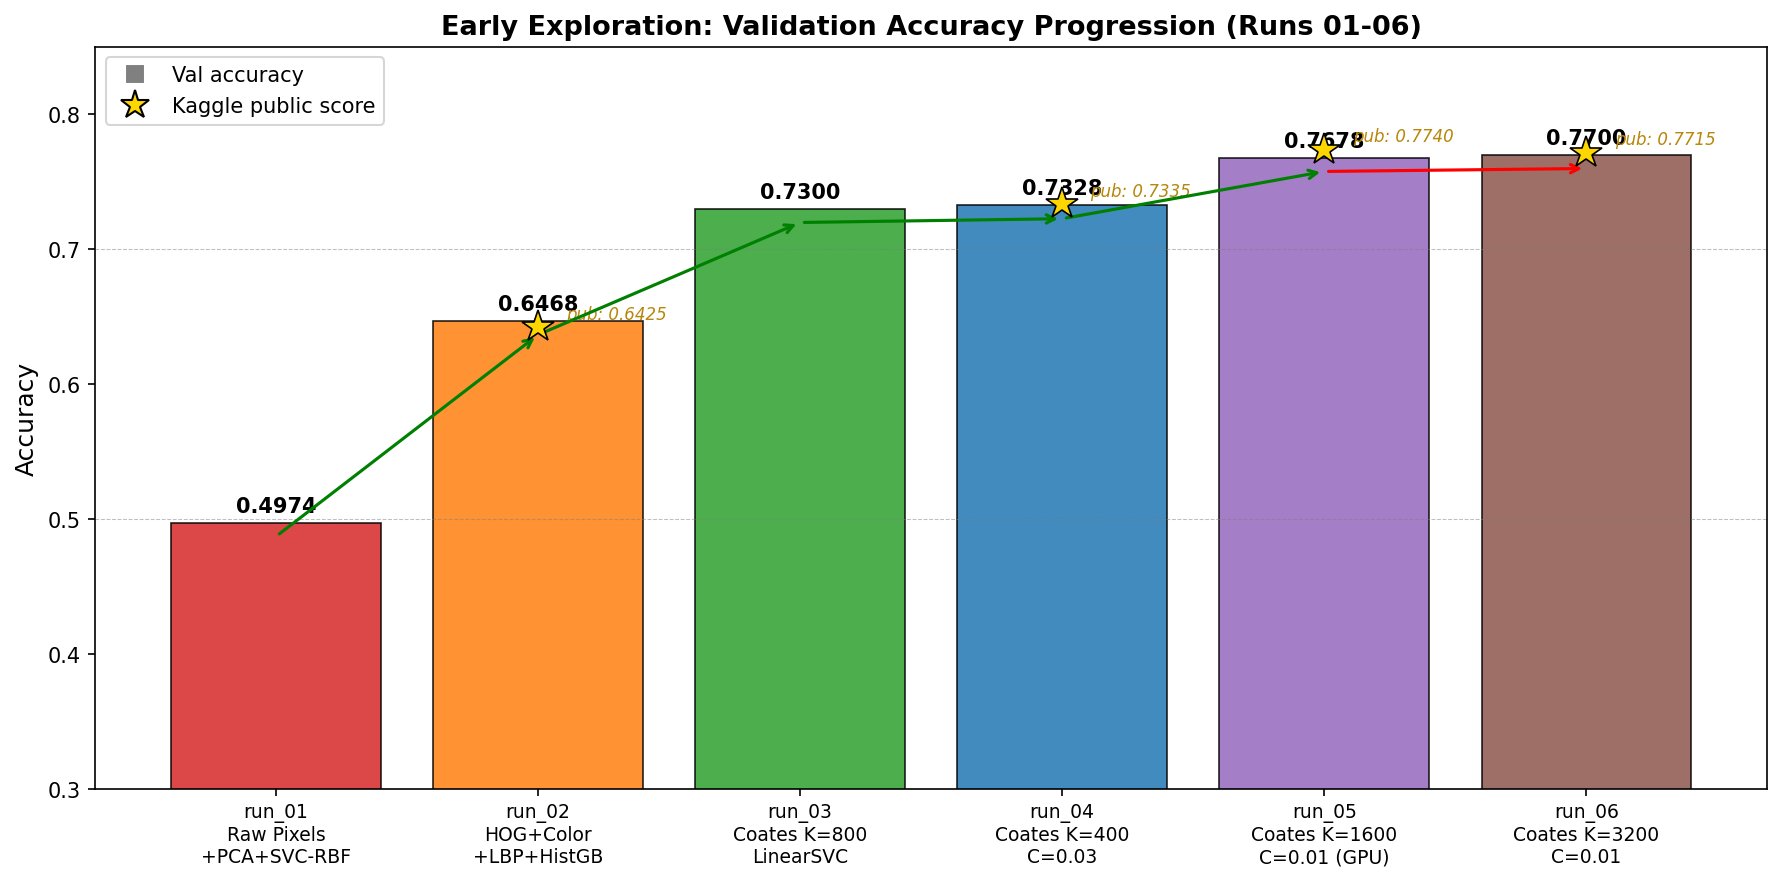
\includegraphics[width=0.85\linewidth]{figures/early_01_progression.png}
  \caption{Validation accuracy progression across runs 01--06, showing the
  transition from raw pixels to handcrafted features to learned features.}
  \label{fig:early_progression}
\end{figure}

\paragraph{Run 01: Raw Pixel Baseline (val 0.497).}
Flatten $32 \times 32 \times 3$ images into 3,072-dim vectors, apply
StandardScaler and PCA (200 components, retaining 94.96\% of variance), then
classify with five standard models.  SVC-RBF achieved the best accuracy of
0.497, while KNN scored only 0.359.

\paragraph{Run 02: Handcrafted Features (val 0.647, public 0.643).}
Replace raw pixels with domain-knowledge-driven descriptors: HOG (grayscale and
per-channel), 16-bin colour histograms, and LBP histograms, totalling
$\sim\!1{,}354$ dimensions.  HistGradientBoosting achieved the best accuracy.
The +0.15 gain over raw pixels came from features that encode local structure.

\paragraph{Runs 03--06: Coates--Ng Feature Learning (val 0.50--0.77).}
We implemented the pipeline described in Section~\ref{sec:coates} and
progressively scaled it:

\begin{table}[H]
\centering
\caption{Progressive scaling of the Coates--Ng pipeline in Phase 1.}
\label{tab:phase1_coates}
\begin{tabular}{@{}llccccl@{}}
\toprule
Run & $K$ & $P$ & Hardware & Best Val & Public & Key Change \\
\midrule
03 & 800  & 6 & CPU & $\sim$0.73 & ---    & First implementation \\
04 & 400--1600 & 6, 8 & CPU & 0.754 & 0.734 & $K/P/C$ sweep (30 configs) \\
05 & 1600 & 6 & GPU & 0.768 & \textbf{0.774} & GPU-accelerated encoding \\
06 & 3200 & 6 & GPU & ---   & 0.772 & Diminishing returns \\
\bottomrule
\end{tabular}
\end{table}

Key findings: (i) learned features massively outperform handcrafted ones
(+0.08 from HOG to Coates $K\!=\!800$); (ii) dictionary size $K$ is the most
important hyperparameter; (iii) optimal regularisation $C$ shifts inversely
with $K$; (iv) diminishing returns appear above $K\!=\!1600$ at the same $C$.

\subsection{Phase 2: Large-Scale Hyperparameter Sweep (run 07)}
\label{sec:phase2}

With the Coates--Ng pipeline validated, we launched a comprehensive
250-configuration grid search on a rented RTX 5090 (32\,GB VRAM):
\[
  P \in \{4, 5, 6, 7, 8\}, \quad
  K \in \{400, 800, \ldots, 8000\}, \quad
  C \in \{0.003, 0.005, 0.01, 0.02, 0.03\}.
\]
All configurations share the same validation split for direct comparability.
The classifier was cuML GPU LinearSVC with L-BFGS solver.

\begin{figure}[H]
  \centering
  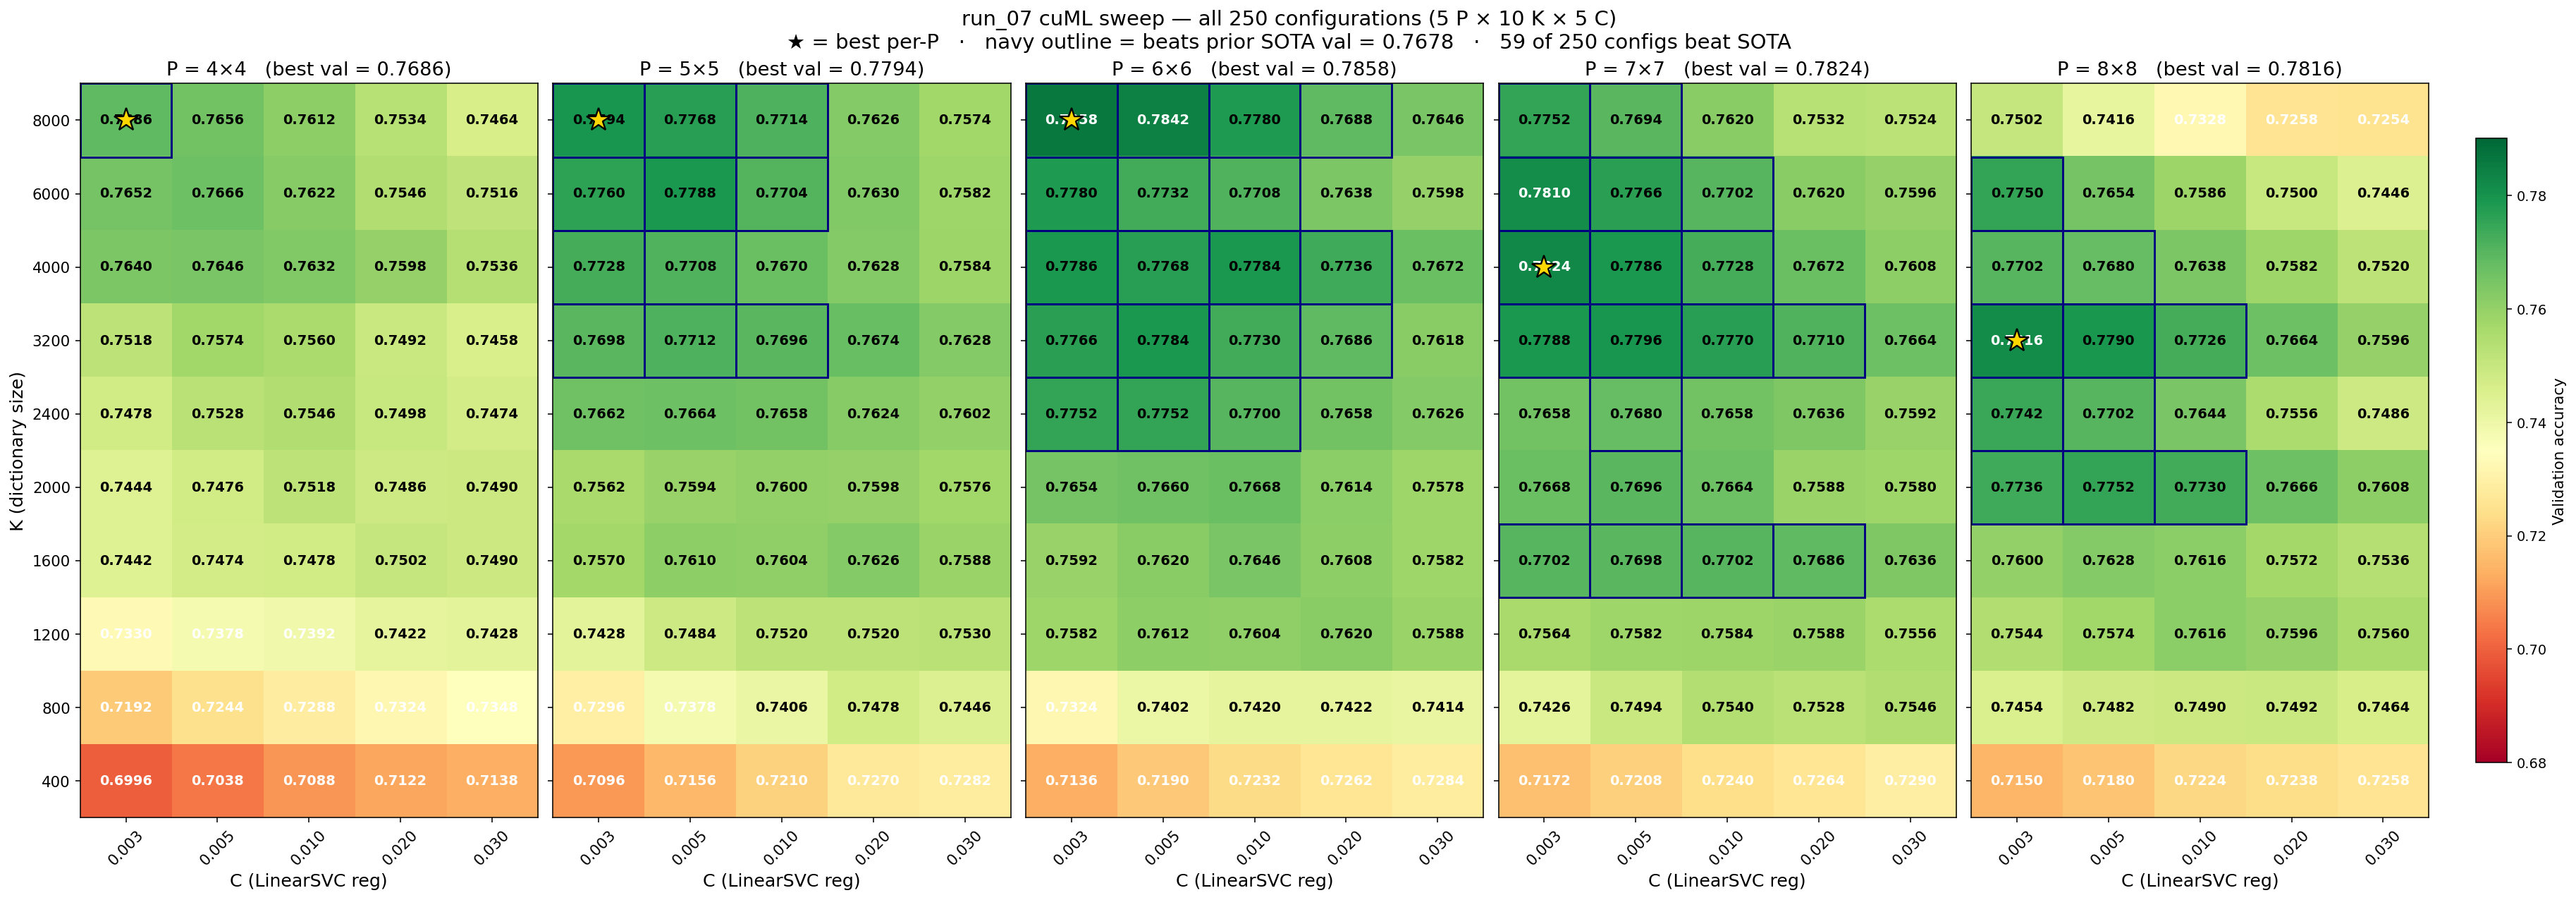
\includegraphics[width=\linewidth]{figures/00_all_250_configs.png}
  \caption{All 250 configurations arranged by patch size, dictionary size, and
  regularisation parameter $C$.}
  \label{fig:all_250}
\end{figure}

\paragraph{Headline result.} Best configuration: $P\!=\!6$, $K\!=\!8000$,
$C\!=\!0.003$---validation 0.7858, public \textbf{0.784} (+1.0\,pp over prior
SOTA).  59 of 250 configs beat the prior val 0.768 baseline.

\paragraph{Key finding: optimal $K$ shrinks as patch size grows.}
This is the most striking pattern in the sweep (Table~\ref{tab:optimal_K},
Figure~\ref{fig:val_vs_K}).  A $P \times P \times 3$ patch lives in a
$3P^2$-dimensional space (48 for $P\!=\!4$, 108 for $P\!=\!6$, 192 for
$P\!=\!8$).  When $K$ exceeds the effective intrinsic dimensionality of the
patch space, additional centroids capture noise rather than structure.

\begin{table}[H]
\centering
\caption{Optimal dictionary size $K^*$ as a function of patch size $P$.}
\label{tab:optimal_K}
\begin{tabular}{@{}cccl@{}}
\toprule
$P$ & Optimal $K$ & Peak Val & Behaviour \\
\midrule
4 & 8000 & 0.769 & Monotonically increasing \\
5 & 8000 & 0.779 & Monotonically increasing \\
6 & \textbf{8000} & \textbf{0.786} & Monotonically increasing, overall winner \\
7 & 4000 & 0.782 & Turns over; $K\!=\!8000$ drops to 0.775 \\
8 & 3200 & 0.782 & Early peak; $K\!=\!8000$ collapses to 0.750 \\
\bottomrule
\end{tabular}
\end{table}

\begin{figure}[H]
  \centering
  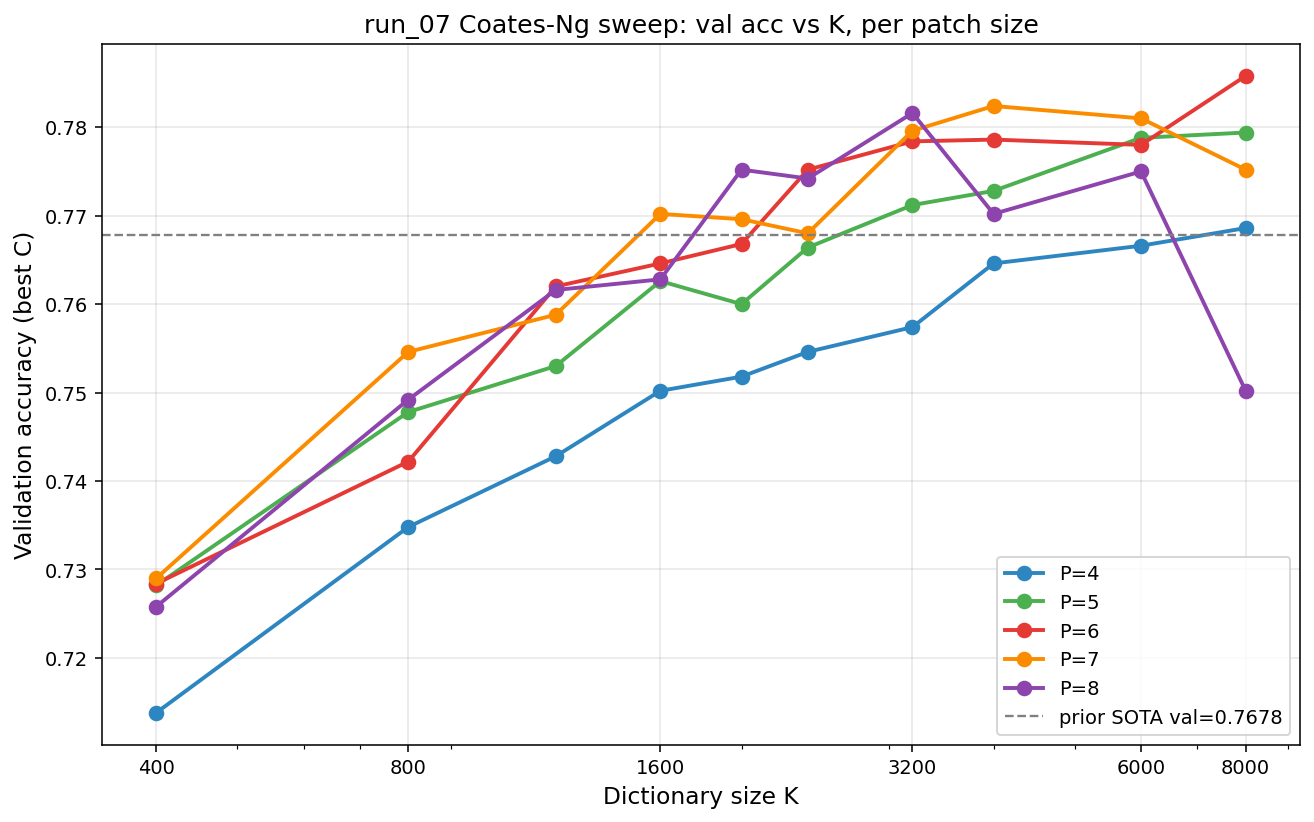
\includegraphics[width=0.85\linewidth]{figures/01_val_vs_K_per_P.png}
  \caption{Validation accuracy vs.\ dictionary size $K$ for each patch size
  $P$, showing the inverse relationship between optimal $K$ and $P$.}
  \label{fig:val_vs_K}
\end{figure}

\begin{figure}[H]
  \centering
  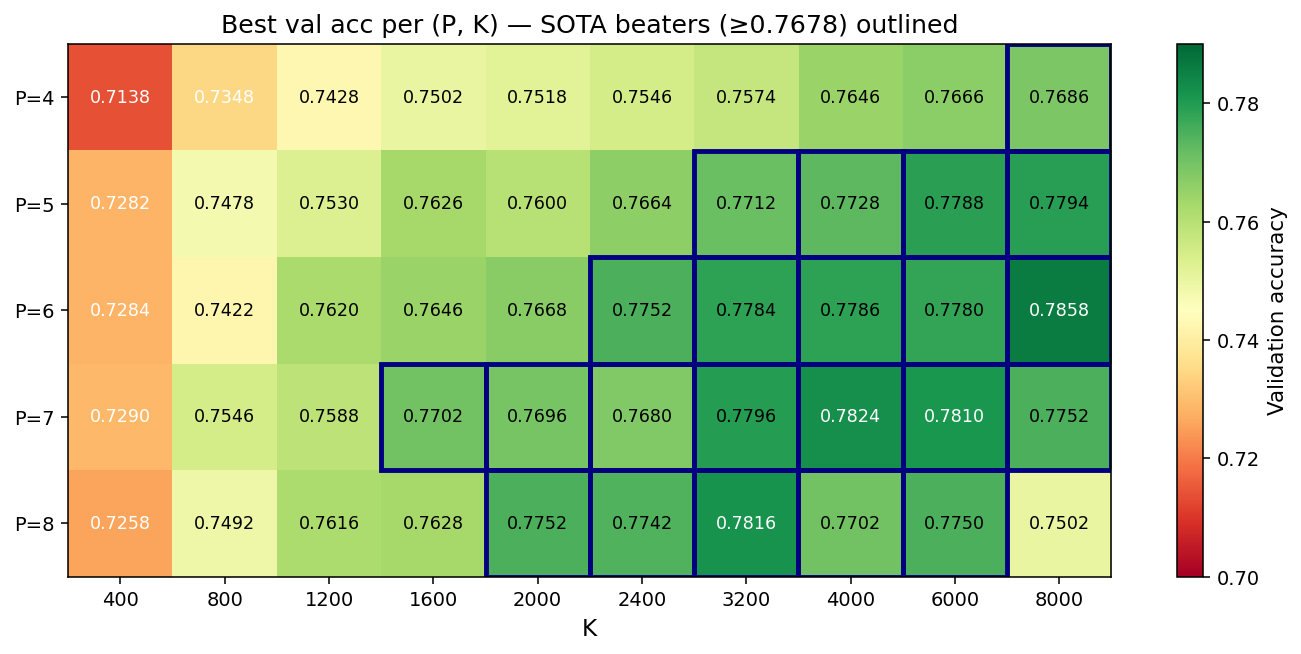
\includegraphics[width=0.75\linewidth]{figures/02_heatmap_best_per_PK.png}
  \caption{$P \times K$ heatmap of best validation accuracy.  $P\!=\!6$
  dominates: 9 of 10 $K$ values beat the prior SOTA.}
  \label{fig:heatmap_PK}
\end{figure}

\subsection{Phase 3: Fine-Grained Optimisation (runs 08, 10)}
\label{sec:phase3}

\paragraph{Phase B: Lower $C$ extension (run 08).}
Since 16 of 50 $(P, K)$ cells had $C\!=\!0.003$ as their best value---the grid
floor---we extended the $C$ grid downward to $\{0.0005, 0.001, 0.002\}$ for
these cells (48 new evaluations).  Only $P\!=\!7$ and $P\!=\!8$ benefited from
lower $C$; smaller patches were already well-served by $C\!=\!0.003$.

The best new result was $P\!=\!6$, $K\!=\!8000$, $C\!=\!0.002$ (val 0.784,
public \textbf{0.788}).  A surprise finding: this configuration scored lower on
validation than $C\!=\!0.003$ (0.784 vs.\ 0.786) but higher on the public
leaderboard (0.788 vs.\ 0.784)---our first concrete evidence that the
5,000-image validation set can disagree with the test set about which model is
better.

\begin{figure}[H]
  \centering
  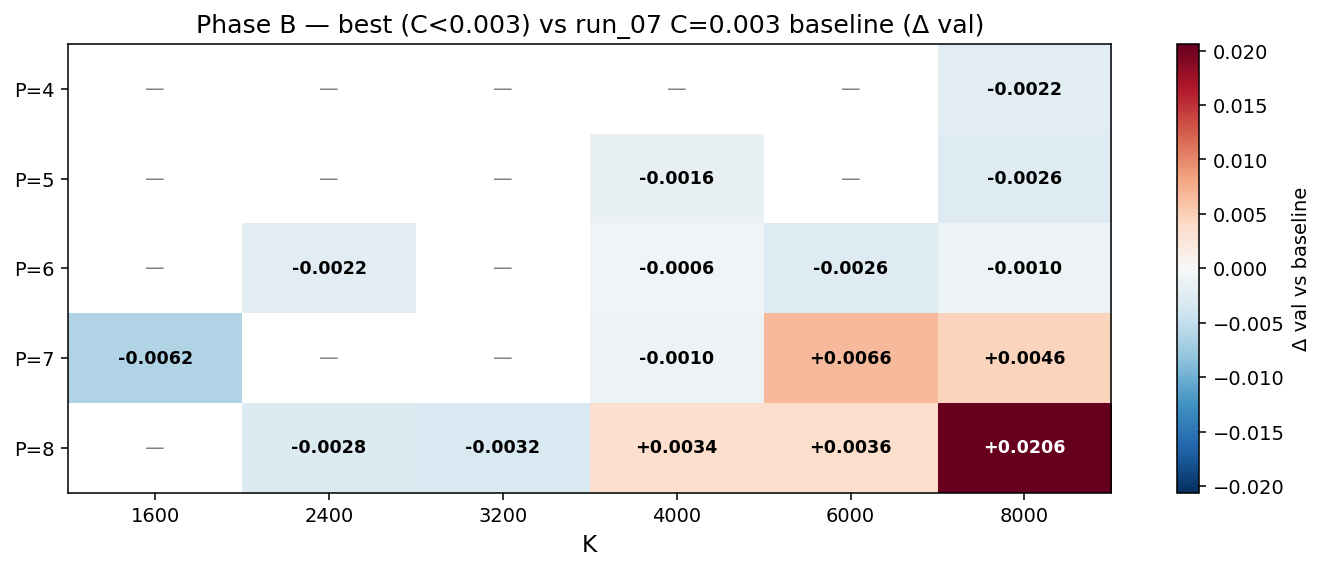
\includegraphics[width=0.75\linewidth]{figures/phase_b_02_delta_heatmap.png}
  \caption{Phase B delta heatmap showing improvement from extending the $C$
  grid below 0.003.  Larger patch sizes benefit most from weaker
  regularisation.}
  \label{fig:phase_b_delta}
\end{figure}

\paragraph{Phase A: Pushing $K$ past 8000 (run 10).}
We tested $K \in \{10000, 12000, 14000\}$ for $P\!=\!6$ with appropriately
lower $C$.  Results: $K\!=\!10000$ matched $K\!=\!8000$ within noise
($\Delta = +0.0002$); $K\!=\!12000$ and $K\!=\!14000$ declined.  The
$K$-to-$C^*$ inverse relationship held perfectly, but beyond $K\!=\!8000$ even
optimally-tuned $C$ could not compensate for increasingly sparse features.

\begin{figure}[H]
  \centering
  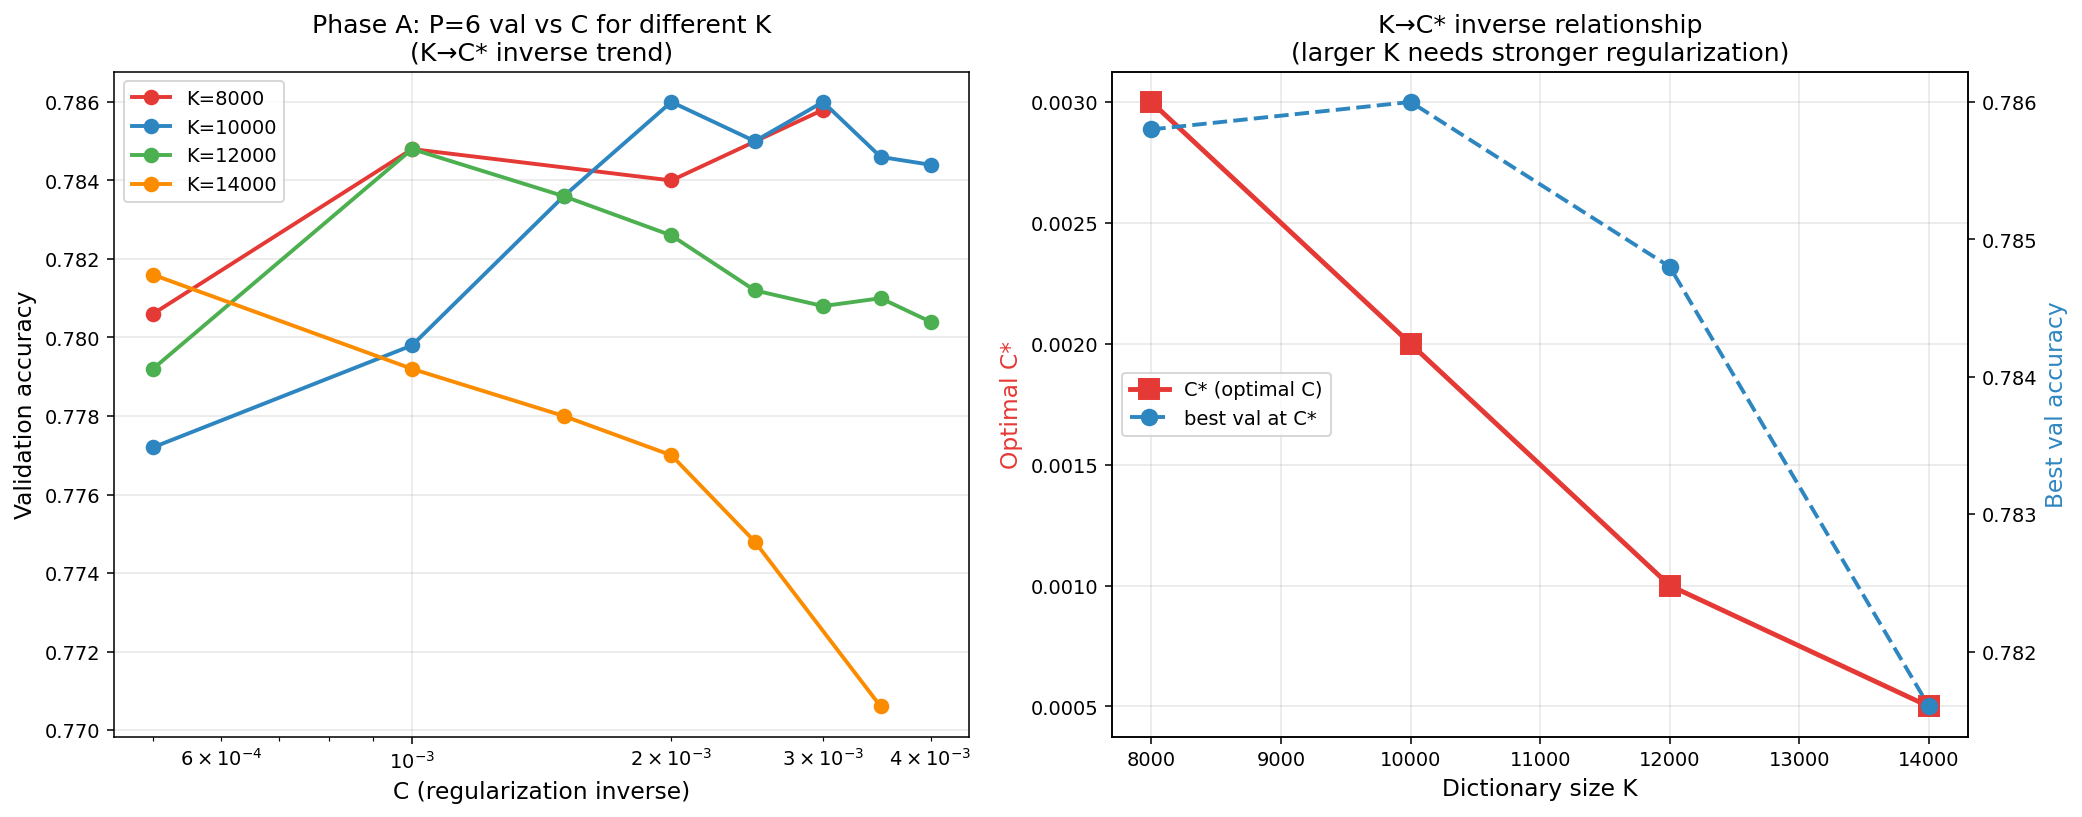
\includegraphics[width=0.75\linewidth]{figures/post07_02_phase_a_analysis.png}
  \caption{Phase A: validation accuracy vs.\ $K$ with optimal $C$.
  $K\!=\!8000$--$10000$ is the plateau for $P\!=\!6$.}
  \label{fig:phase_a}
\end{figure}

\textbf{Conclusion:} The Coates--Ng pipeline reached its ceiling from a
hyperparameter perspective at $K\!=\!8000$ for $P\!=\!6$.  Further improvement
required fundamentally different approaches.

\subsection{Phase 4: Augmentation and Normalisation (runs 12--19)}
\label{sec:phase4}

This was the breakthrough phase, where we shifted from hyperparameter tuning to
data augmentation, feature engineering, and ensembling.

\paragraph{Flip augmentation (run 12): the biggest single win.}
Doubling the training set via horizontal flip with TTA-2 at test time produced
+0.028 on the public leaderboard (Table~\ref{tab:flip}).  This single change
produced more improvement than all hyperparameter tuning combined.

\begin{table}[H]
\centering
\caption{Impact of horizontal flip augmentation.}
\label{tab:flip}
\begin{tabular}{@{}llccc@{}}
\toprule
Configuration & Augmentation & Val & Public & $\Delta$ Public \\
\midrule
$P\!=\!6$, $K\!=\!8000$, $C\!=\!0.002$ & None & 0.784 & 0.788 & --- \\
$P\!=\!6$, $K\!=\!8000$, $C\!=\!0.002$ & \textbf{Flip + TTA-2} & \textbf{0.812} & \textbf{0.816} & \textbf{+0.028} \\
\bottomrule
\end{tabular}
\end{table}

\begin{figure}[H]
  \centering
  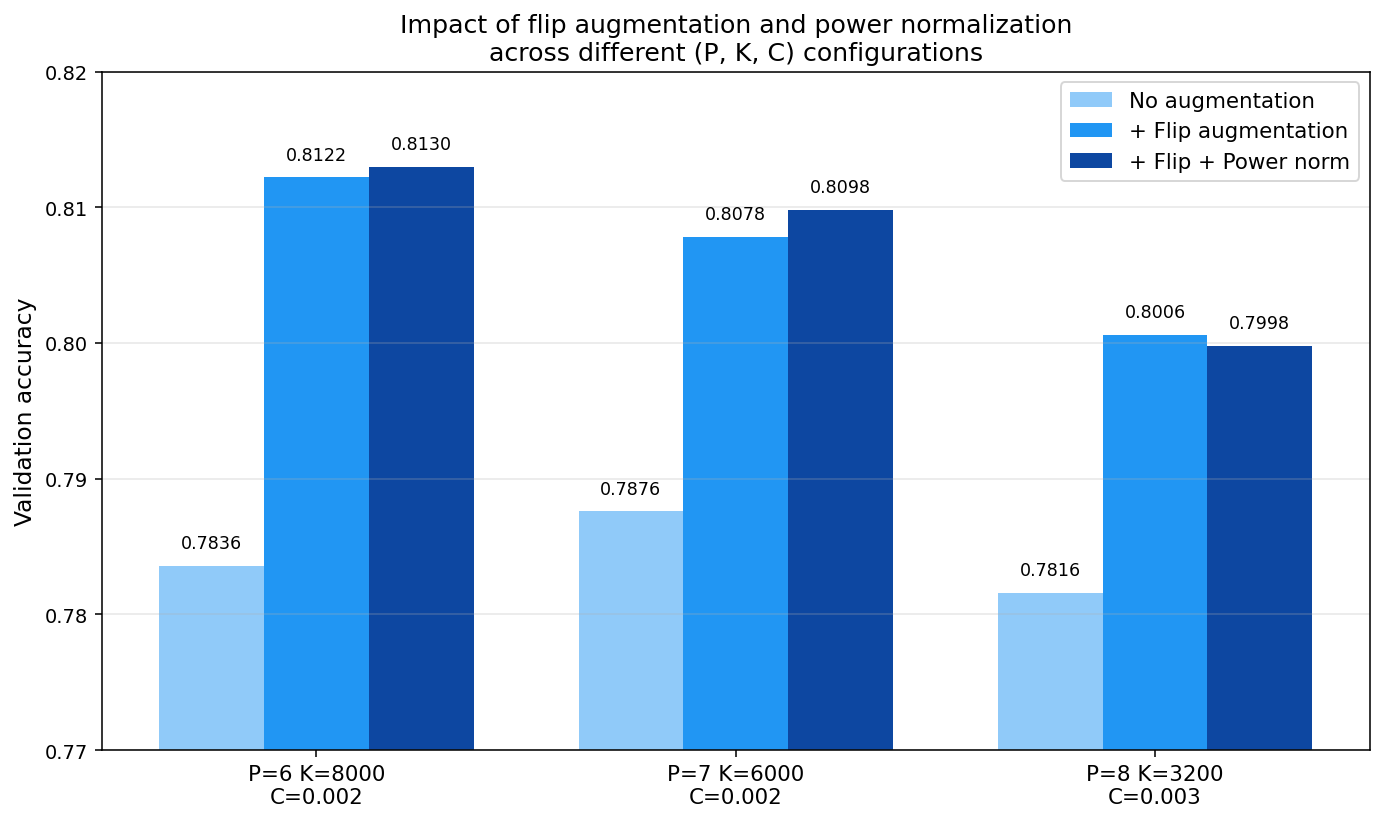
\includegraphics[width=0.85\linewidth]{figures/post07_03_flip_pnorm_impact.png}
  \caption{Impact of flip augmentation and power normalisation on both
  validation and public leaderboard scores.}
  \label{fig:flip_pnorm}
\end{figure}

Why so effective?  Several factors converge: (i) the sample-to-dimension ratio
improves from 1.56 to 3.125 for the 32,000-dim feature space; (ii) all 10
classes are horizontally symmetric, so the flip is label-preserving; (iii)
TTA-2 reduces prediction variance without introducing bias; (iv) the pipeline
was fundamentally data-starved.

\paragraph{Power normalisation (run 17): the second breakthrough.}
Applying signed square-root compression (Section~\ref{sec:powernorm}) improved
the public score by +0.012 despite only +0.002 on validation.  This 6.4$\times$
ratio between public and val gains suggests that power normalisation
improves generalisation far more than the small validation set can measure.

\begin{figure}[H]
  \centering
  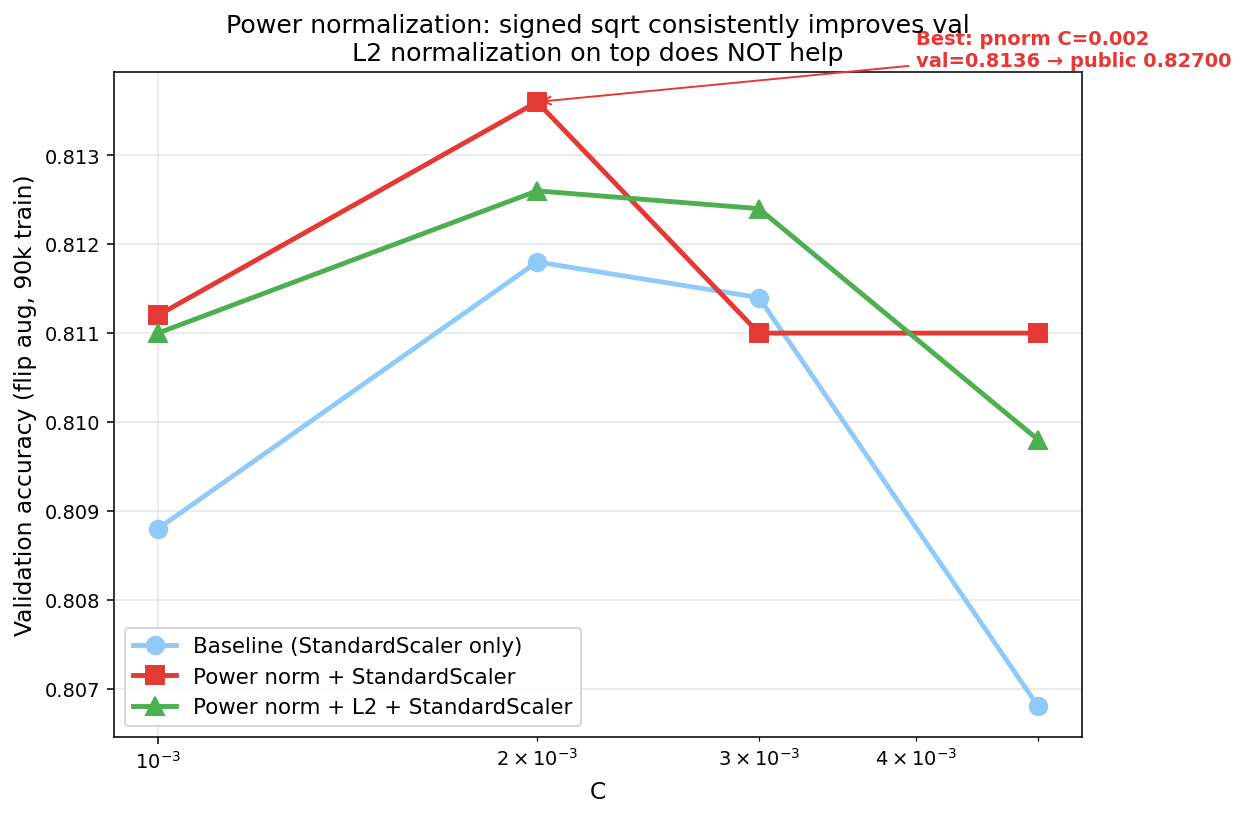
\includegraphics[width=0.85\linewidth]{figures/post07_04_power_norm_comparison.png}
  \caption{Power normalisation: feature distribution before and after
  transformation, and accuracy comparison.}
  \label{fig:power_norm}
\end{figure}

\paragraph{Failed experiments.}
Several experiments after the flip augmentation breakthrough did not improve
results (Figure~\ref{fig:failed}).  Each failure was instructive:

\begin{itemize}[nosep]
  \item \textbf{Random crops (run 13):} OOM at $4\times$ augmentation
        ($200\text{k} \times 32\text{k}$ float32 exceeds 32\,GB VRAM), or
        regression when replacing originals with crops (val 0.791 vs.\ 0.812
        due to train--test distribution mismatch).
  \item \textbf{10-view TTA (run 14):} Public dropped to 0.800 ($-0.016$).
        Corner crops on $32 \times 32$ images shift objects out of frame and
        disrupt quadrant features.
  \item \textbf{Two-layer Coates (run 16):} With $K_1\!=\!1600$, the first
        layer is too weak; larger $K_1$ requires ZCA on $>$36,000-dim
        vectors---computationally impractical.
  \item \textbf{Multi-crop feature averaging (run 18):} Val dropped from 0.814
        to 0.808.  Averaging across shifted crops blurs spatial information.
\end{itemize}

\textbf{Common lesson:} Spatial manipulations on $32 \times 32$ images with
quadrant pooling are net harmful.  The only safe augmentation is horizontal
flip, which preserves the vertical axis structure.

\begin{figure}[H]
  \centering
  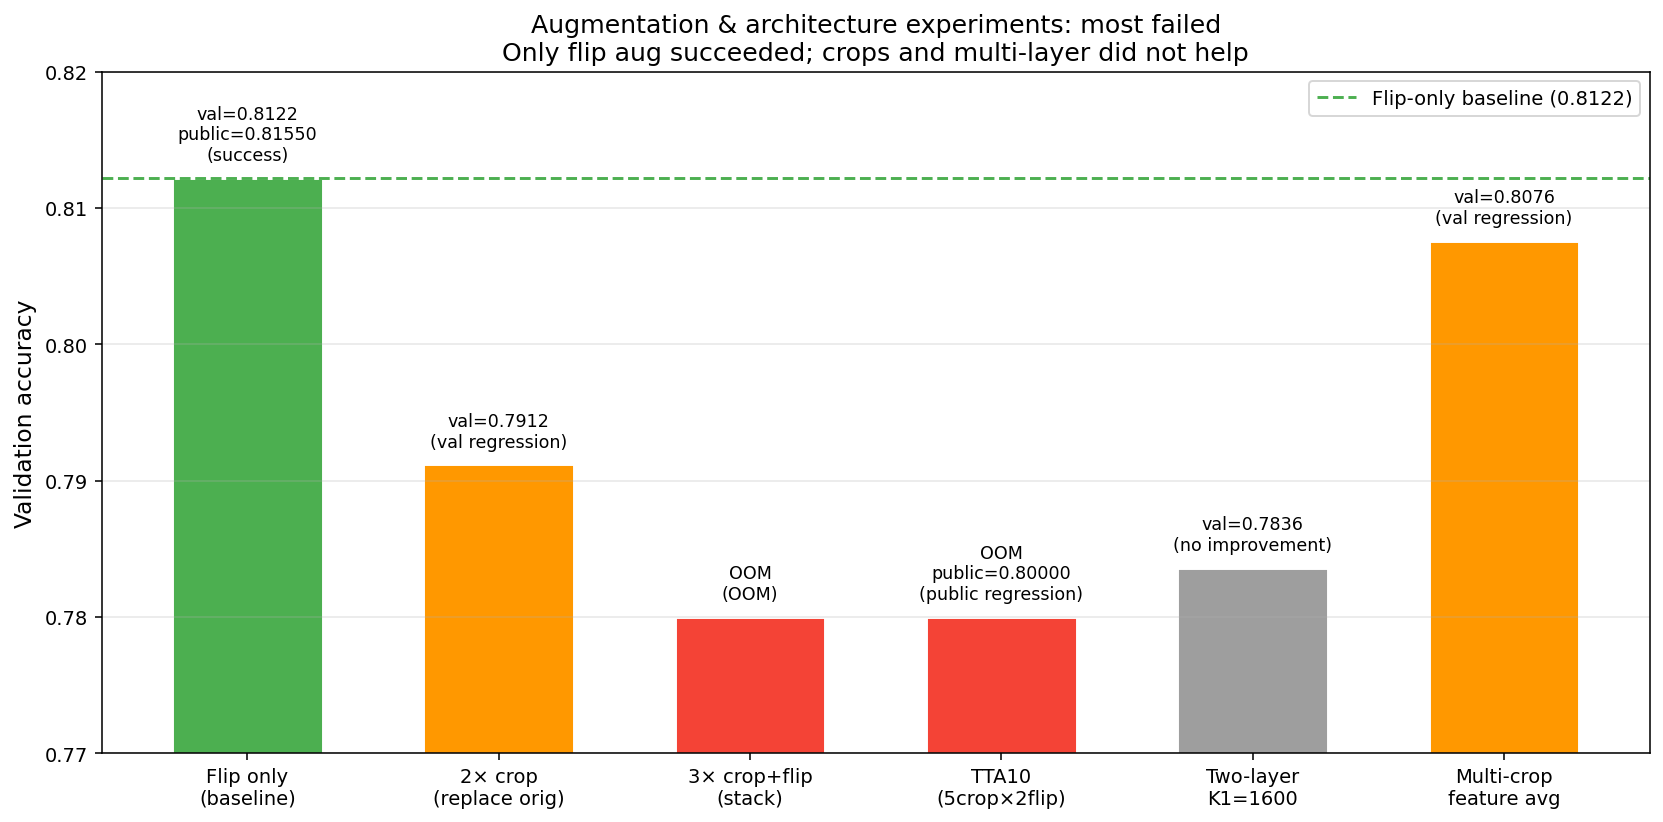
\includegraphics[width=0.85\linewidth]{figures/post07_05_failed_experiments.png}
  \caption{Summary of failed experiments showing that spatial augmentations on
  $32 \times 32$ images with quadrant pooling are destructive.}
  \label{fig:failed}
\end{figure}

\paragraph{Multi-$P$ ensemble (run 19): the final piece.}
Ensembling models with the same $P$ is useless (86\% prediction agreement), but
models with different patch sizes produce genuinely different features.  The
two-model ensemble ($P\!=\!6$ + $P\!=\!7$) gained +0.010 on validation;
adding $P\!=\!8$ contributed only +0.0002 (2 additional correct predictions),
so the two-model ensemble was selected for parsimony.

\begin{figure}[H]
  \centering
  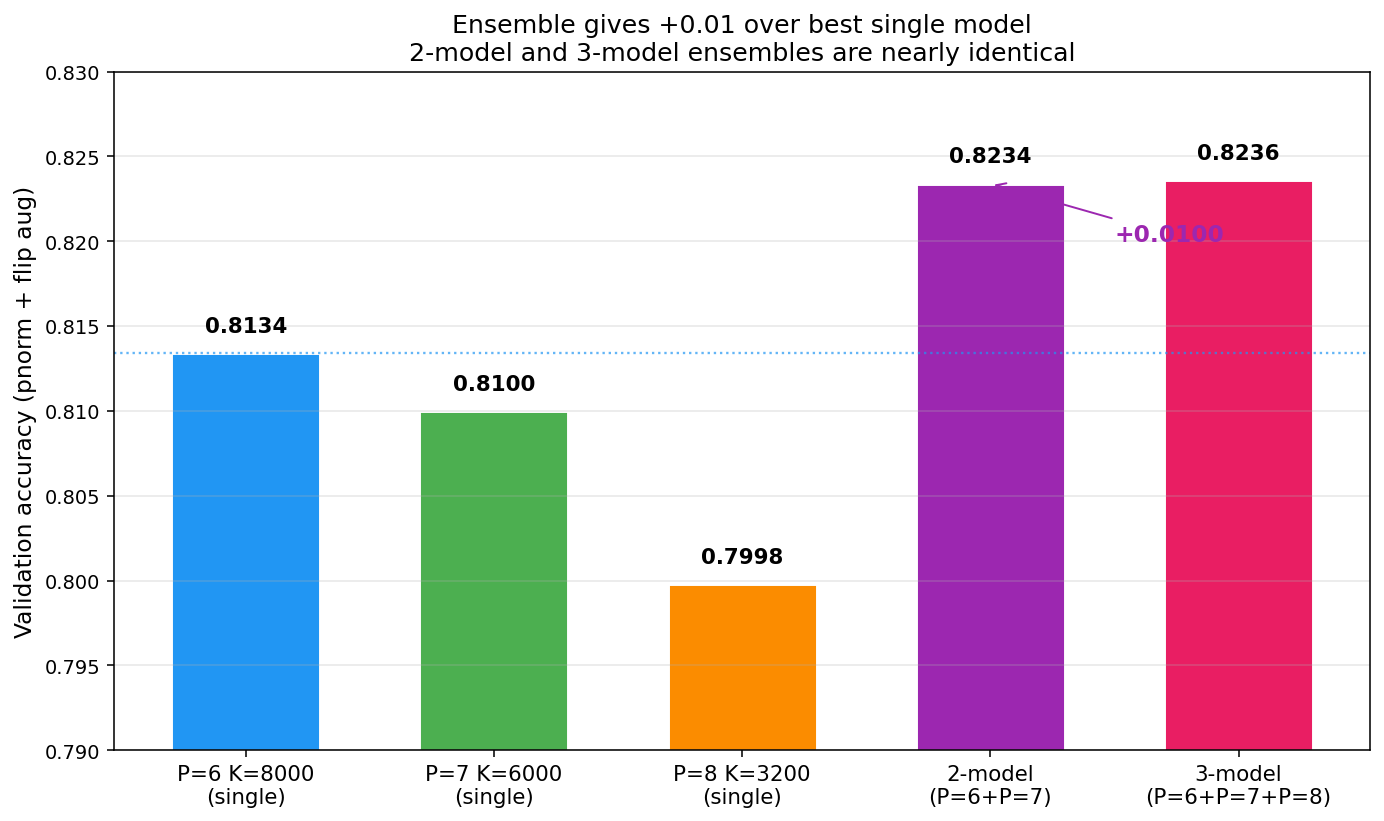
\includegraphics[width=0.85\linewidth]{figures/post07_06_ensemble_comparison.png}
  \caption{Ensemble comparison: individual models, two-model ($P\!=\!6 +
  P\!=\!7$), and three-model ensembles.}
  \label{fig:ensemble}
\end{figure}

% =============================================================================
% 5. RESULTS
% =============================================================================
\section{Results}
\label{sec:results}

\subsection{Classifier Comparison}
\label{sec:classifier_comparison}

The assignment requires comparison of at least two classifiers.  Across our 19
runs, we evaluated a wide range of classifiers under different feature
representations.  Table~\ref{tab:classifier_comparison} summarises the
progression, demonstrating that \textbf{feature quality is far more important
than classifier choice}.

\begin{table}[H]
\centering
\caption{Classifier comparison across feature representations.  Moving from raw
pixels to Coates features gained +0.29 in accuracy, while the best classifier
changed from nonlinear (SVC-RBF) to linear (LinearSVC).}
\label{tab:classifier_comparison}
\begin{tabular}{@{}p{4.2cm}p{2.4cm}lcc@{}}
\toprule
Feature Representation & Dims & Classifier & Val & Public \\
\midrule
Raw pixels + PCA(200) & 200 & SVC-RBF & 0.497 & --- \\
HOG + Colour + LBP & 1,354 & HistGradientBoosting & 0.647 & 0.643 \\
Coates $K\!=\!1600$, $P\!=\!6$ & 6,400 & LinearSVC & 0.768 & 0.774 \\
Coates $K\!=\!8000$, $P\!=\!6$ & 32,000 & cuML LinearSVC & 0.786 & 0.784 \\
\quad + flip augmentation & 32,000 & cuML LinearSVC & 0.812 & 0.816 \\
\quad + power normalisation & 32,000 & cuML LinearSVC & 0.814 & 0.827 \\
\quad + 2-model ensemble & 32k + 24k & cuML LinearSVC $\times 2$ & 0.823 & \textbf{0.829} \\
\bottomrule
\end{tabular}
\end{table}

Within the raw pixel representation, the 0.14 gap between SVC-RBF (0.497) and
KNN (0.359) shows that classifier choice matters when features are poor.
Within the handcrafted feature representation, the gap narrows to 0.09 (HistGB
0.647 vs.\ LogReg 0.555).  Within the Coates pipeline, LinearSVC is both
faster and better than nonlinear alternatives because the features are designed
to be linearly separable.

\subsection{Ablation Study}
\label{sec:ablation}

Table~\ref{tab:ablation} isolates the contribution of each component by adding
them incrementally to the best base configuration.

\begin{table}[H]
\centering
\caption{Ablation study: contribution of each component added to the baseline
$P\!=\!6$, $K\!=\!8000$, $C\!=\!0.002$ configuration.}
\label{tab:ablation}
\begin{tabular}{@{}lccc@{}}
\toprule
Component & Val & Public & $\Delta$ Public \\
\midrule
Baseline ($K\!=\!8000$, $C\!=\!0.002$) & 0.784 & 0.788 & --- \\
+ Flip augmentation & 0.812 & 0.816 & +0.028 \\
+ Power normalisation & 0.814 & 0.827 & +0.012 \\
+ 2-model ensemble + TTA & 0.823 & 0.829 & +0.002 \\
\bottomrule
\end{tabular}
\end{table}

The ablation reveals a clear hierarchy: flip augmentation contributes the most
(+0.028), followed by power normalisation (+0.012) and ensembling (+0.002).
Collectively, these data- and feature-level improvements contribute +0.042 on
the public leaderboard, far exceeding the +0.014 from all hyperparameter
tuning in Phases 2--3.

\subsection{Validation vs.\ Public Score Analysis}
\label{sec:val_vs_public}

A recurring theme throughout this project was the unreliability of validation
accuracy as a predictor of public leaderboard performance.

\begin{figure}[H]
  \centering
  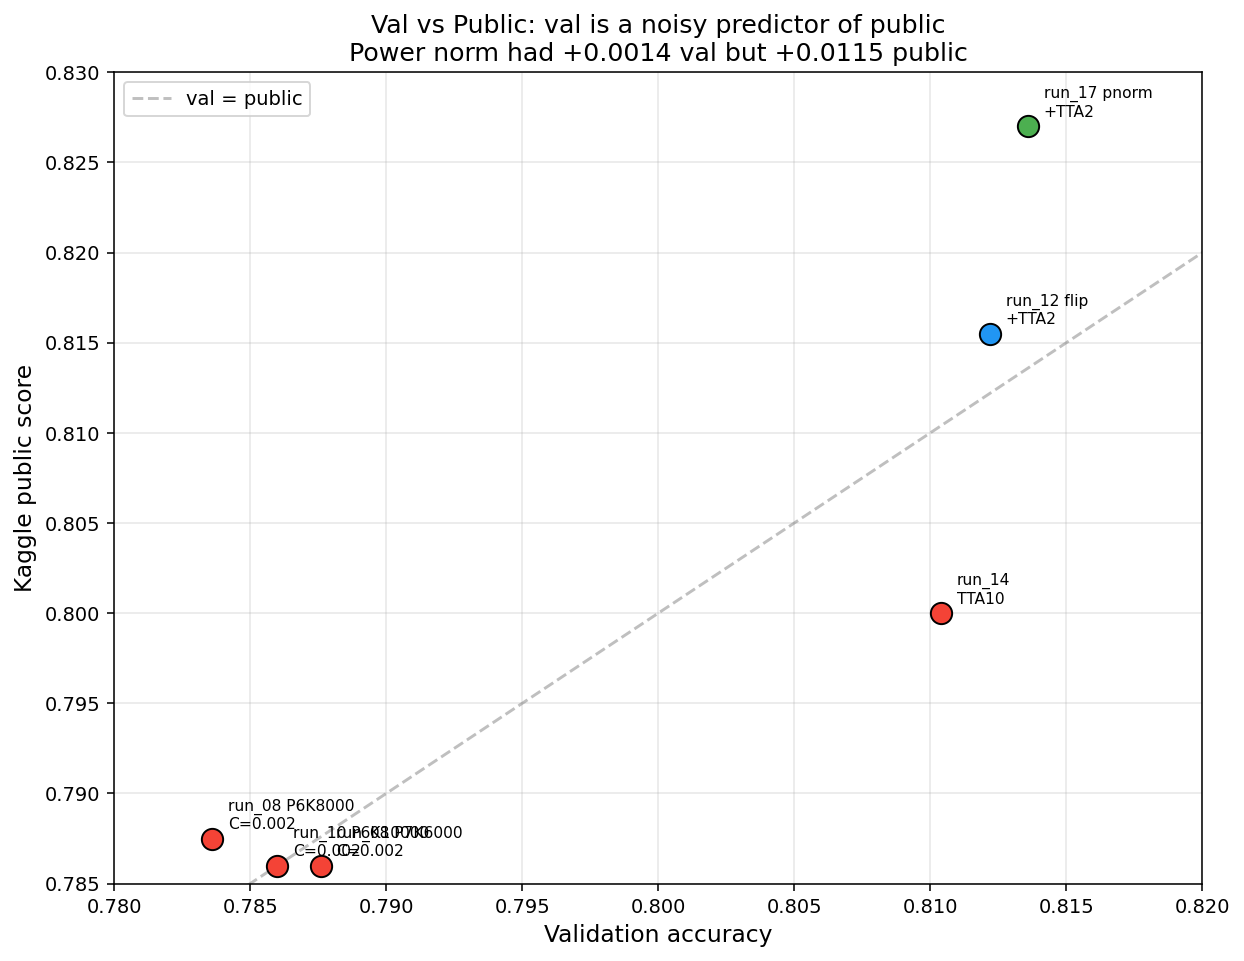
\includegraphics[width=0.85\linewidth]{figures/post07_07_val_vs_public.png}
  \caption{Scatter plot of validation accuracy vs.\ public leaderboard score
  across all submitted configurations.}
  \label{fig:val_vs_public}
\end{figure}

Notable discrepancies include:

\begin{itemize}[nosep]
  \item $C\!=\!0.002$ scored lower on val than $C\!=\!0.003$ (0.784 vs.\
        0.786) but higher on public (0.788 vs.\ 0.784).
  \item Power normalisation gained +0.002 on val but +0.012 on public (a
        $6.4\times$ ratio).
  \item 10-view TTA showed decent val (0.810) but poor public (0.800).
\end{itemize}

With a 5,000-image validation set, the standard error is approximately
$\sqrt{0.8 \times 0.2 / 5000} \approx 0.006$.  Validation differences below
0.005 are essentially noise.  The practical lesson: after basic hyperparameter
selection on validation, prioritise techniques that improve generalisation
(augmentation, normalisation) over fine-grained accuracy chasing.

% =============================================================================
% 6. FINAL SOLUTION
% =============================================================================
\section{Final Solution}
\label{sec:final}

\subsection{Complete Pipeline}

The final solution is a two-model ensemble where each model follows the same
pipeline with different patch and dictionary sizes:

\begin{itemize}[nosep]
  \item \textbf{Model A:} $P = 6$, $K = 8000$, $C = 0.002$ (32,000-dim features)
  \item \textbf{Model B:} $P = 7$, $K = 6000$, $C = 0.002$ (24,000-dim features)
\end{itemize}

For each model:
\begin{enumerate}[nosep]
  \item \textit{Dictionary learning:} Sample $10^6$ patches $\to$ contrast
        normalisation $\to$ ZCA whitening $\to$ MiniBatchKMeans.
  \item \textit{Feature extraction:} Stride-1 patches $\to$ contrast norm
        $\to$ ZCA projection $\to$ triangle encoding $\to$ $2 \times 2$
        quadrant pooling.
  \item \textit{Augmentation:} Append horizontally flipped training images
        (100k total).
  \item \textit{Normalisation:} Power norm $\to$ StandardScaler.
  \item \textit{Training:} cuML LinearSVC ($C = 0.002$, squared hinge, L2).
  \item \textit{TTA-2:} Average \texttt{decision\_function} from original and
        flipped test views.
\end{enumerate}

\noindent\textbf{Ensemble:} Average per-model TTA-2 scores (soft voting),
then argmax.

\subsection{Component Contributions}

Table~\ref{tab:contributions} summarises why each component matters, with
the experimental evidence supporting its inclusion.

\begin{table}[H]
\centering
\caption{Contribution of each pipeline component.}
\label{tab:contributions}
\begin{tabular}{@{}lll@{}}
\toprule
Component & Contribution & Evidence \\
\midrule
Coates--Ng features & +0.27 over raw pixels & run 01 vs.\ 05 \\
$K\!=\!8000$ dictionary & +0.05 over $K\!=\!1600$ & run 05 vs.\ 07 \\
Flip augmentation & +0.028 public & run 08 vs.\ 12 \\
Power normalisation & +0.012 public & run 12 vs.\ 17 \\
2-model ensemble & +0.010 val & run 17 vs.\ 19 \\
\bottomrule
\end{tabular}
\end{table}

\subsection{Final Results}

\begin{table}[H]
\centering
\begin{tabular}{@{}lc@{}}
\toprule
Metric & Value \\
\midrule
Validation accuracy (5k holdout) & \textbf{0.8234} \\
Public leaderboard & \textbf{0.8290} \\
Leaderboard position & \textbf{1st place} \\
\bottomrule
\end{tabular}
\end{table}

% =============================================================================
% 7. OVERALL PROGRESSION
% =============================================================================

Figure~\ref{fig:progression} shows the overall public leaderboard score
progression across all phases.

\begin{figure}[H]
  \centering
  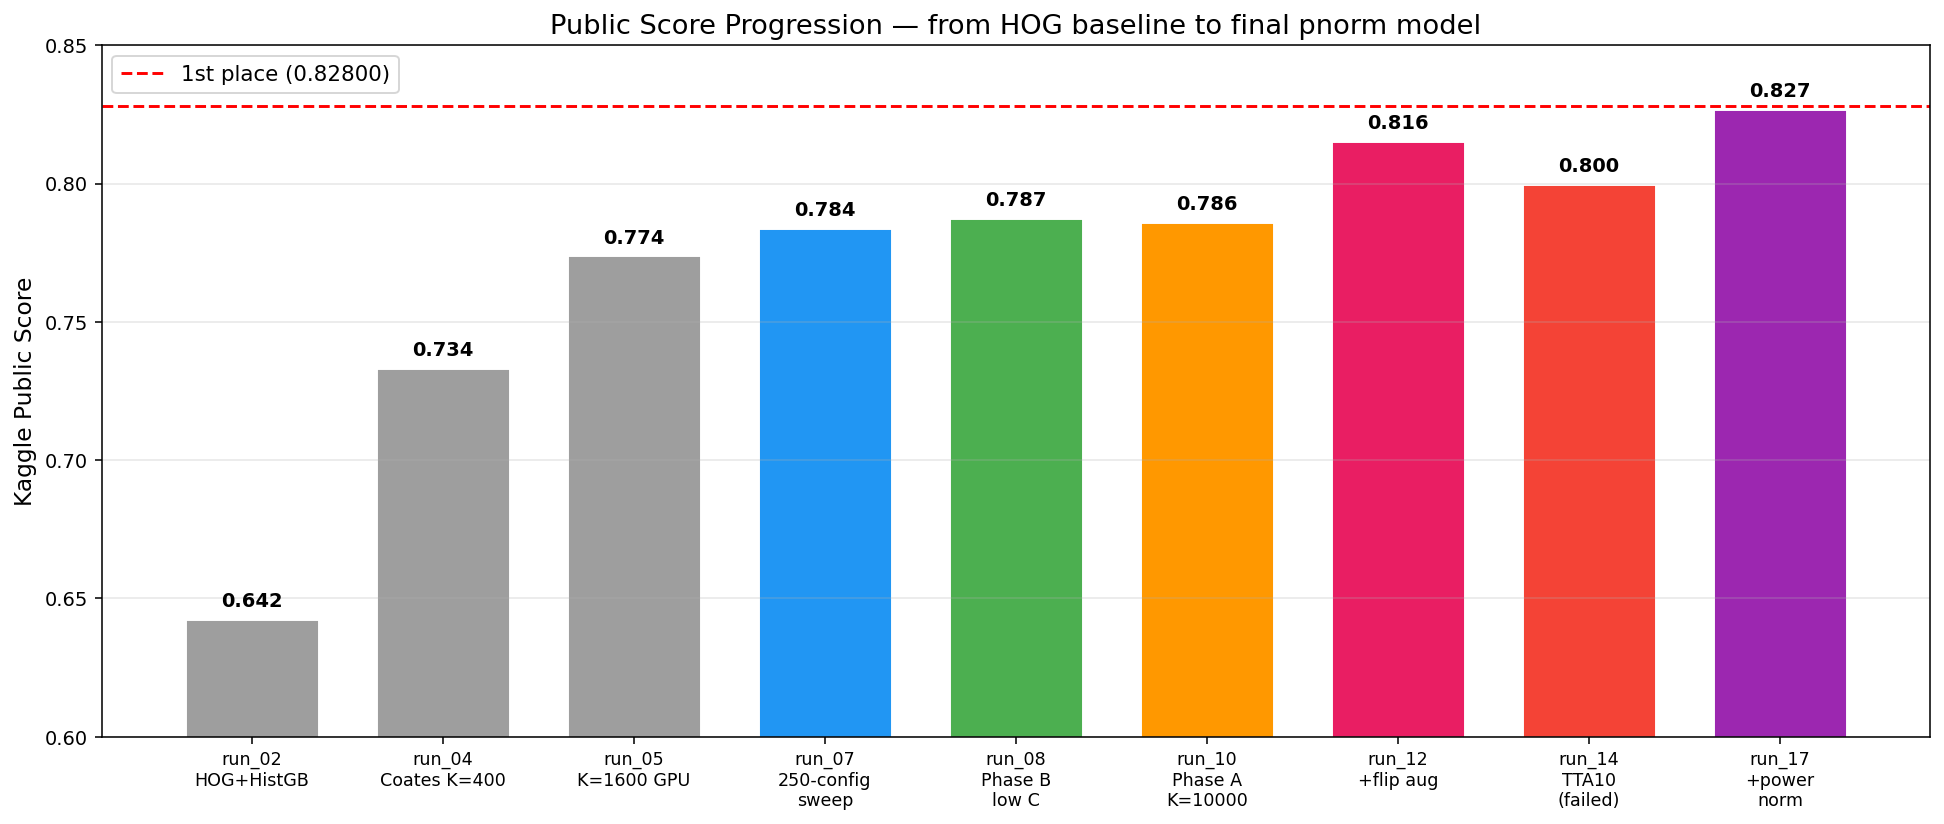
\includegraphics[width=\linewidth]{figures/post07_01_public_progression.png}
  \caption{Public leaderboard score progression across all experimental
  phases, from initial submission (0.643) to final ensemble (0.829).}
  \label{fig:progression}
\end{figure}

% =============================================================================
% 8. CONCLUSION
% =============================================================================
\section{Conclusion}
\label{sec:conclusion}

\subsection{Summary}

This project traced a path through four distinct phases of optimisation:

\begin{table}[H]
\centering
\caption{Summary of the four experimental phases.}
\label{tab:phases}
\begin{tabular}{@{}llccc@{}}
\toprule
Phase & Key Activity & Public & $\Delta$ \\
\midrule
1. Architecture (runs 01--06) & Raw pixels $\to$ Coates--Ng & 0.774 & --- \\
2. HP sweep (run 07) & 250-config grid on GPU & 0.784 & +0.010 \\
3. Fine-tuning (runs 08, 10) & Lower $C$, higher $K$ & 0.788 & +0.004 \\
4. Add-ons (runs 12--19) & Flip, pnorm, ensemble & \textbf{0.829} & +0.041 \\
\bottomrule
\end{tabular}
\end{table}

The most important lesson: \textbf{Phases 2 and 3 together gained only +0.014,
while Phase 4 gained +0.041.}  Data augmentation (+0.028), feature
normalisation (+0.012), and ensembling (+0.010) collectively contributed far
more than exhaustive hyperparameter tuning.

\subsection{What Worked}

\begin{enumerate}[nosep]
  \item \textbf{Coates--Ng unsupervised feature learning} (+0.27 over raw
        pixels).  Learning features from data with K-Means is far more
        effective than hand-designing them, even with classical tools.
  \item \textbf{Horizontal flip augmentation} (+0.028).  Doubling the training
        set with a label-preserving transformation addresses the fundamental
        data bottleneck.
  \item \textbf{Power normalisation} (+0.012).  A one-line transformation that
        compresses the skewed feature distribution improves generalisation more
        than any amount of hyperparameter tuning.
  \item \textbf{Multi-$P$ ensemble} (+0.010).  Different patch sizes capture
        genuinely different visual information, enabling productive diversity.
\end{enumerate}

\subsection{What Did Not Work}

\begin{itemize}[nosep]
  \item \textbf{$K > 8000$:} Diminishing returns; the 108-dim patch space
        saturates.
  \item \textbf{Spatial crops and multi-view TTA:} Destructive on $32 \times
        32$ images with quadrant pooling.
  \item \textbf{Two-layer Coates:} Scalability trap between first-layer
        quality and second-layer tractability.
  \item \textbf{Feature averaging:} Blurs spatial information that quadrant
        pooling encodes.
\end{itemize}

\subsection{Lessons Learned}

In retrospect, flip augmentation should have been tried immediately after
establishing the Coates--Ng pipeline.  The four-phase journey demonstrates a
common pattern in machine learning projects: researchers spend the majority of
their effort on hyperparameter optimisation when the real gains come from
improving data quality and feature representations.  For classical pipelines
operating under the constraints of this assignment, the hierarchy is clear:
\emph{feature learning method $>$ data augmentation $>$ feature normalisation
$>$ hyperparameter tuning $>$ classifier choice}.

% =============================================================================
% REFERENCES
% =============================================================================
\begin{thebibliography}{9}

\bibitem{coates2011analysis}
A.~Coates, H.~Lee, and A.~Y.~Ng.
\newblock An analysis of single-layer networks in unsupervised feature learning.
\newblock In \emph{Proceedings of the 14th International Conference on
Artificial Intelligence and Statistics (AISTATS)}, pages 215--223, 2011.

\bibitem{coates2011selecting}
A.~Coates and A.~Y.~Ng.
\newblock Selecting receptive fields in deep networks.
\newblock In \emph{Advances in Neural Information Processing Systems (NIPS)},
pages 2528--2536, 2011.

\bibitem{perronnin2010improving}
F.~Perronnin, J.~S\'{a}nchez, and T.~Mensink.
\newblock Improving the {F}isher kernel for large-scale image classification.
\newblock In \emph{European Conference on Computer Vision (ECCV)}, pages
143--156. Springer, 2010.

\end{thebibliography}

% =============================================================================
% APPENDIX
% =============================================================================
\appendix
\section{Full Experimental Timeline}
\label{app:timeline}

Table~\ref{tab:timeline} records the complete experimental timeline with
timestamps, configurations, and results for all milestone runs.

\begin{table}[H]
\centering
\caption{Full experimental timeline (selected milestones).}
\label{tab:timeline}
\small
\begin{tabular}{@{}llp{4.5cm}ccp{3cm}@{}}
\toprule
Time & Run & Configuration & Val & Public & Note \\
\midrule
Apr 11 04:30 & 01 & PCA(200) + SVC-RBF & 0.497 & --- & Raw pixel baseline \\
Apr 11 05:30 & 02 & HOG+Colour+LBP + HistGB & 0.647 & 0.643 & First submission \\
Apr 11 06:18 & 04 & Coates $K\!=\!400$ $P\!=\!6$ & 0.730 & --- & Crossed 0.70 bar \\
Apr 11 08:17 & 05 & Coates $K\!=\!1600$ $P\!=\!6$ GPU & 0.768 & 0.774 & New SOTA \\
Apr 11 15:39 & 06 & Coates $K\!=\!3200$ $P\!=\!6$ & --- & 0.772 & Diminishing returns \\
Apr 11 23:37 & 07 & $K\!=\!8000$ $P\!=\!6$ cuML & 0.786 & 0.784 & 250-config sweep \\
Apr 12 06:28 & 08 & $P\!=\!7$ $K\!=\!6000$ $C\!=\!0.002$ & 0.788 & 0.786 & Phase B \\
Apr 12 07:49 & 08 & $P\!=\!6$ $K\!=\!8000$ $C\!=\!0.002$ & 0.784 & 0.788 & Val--public gap \\
Apr 12 09:45 & 12 & + Flip augmentation & 0.812 & 0.816 & Biggest single win \\
Apr 12 18:13 & 17 & + Power normalisation & 0.814 & 0.827 & Second biggest win \\
Apr 12 20:17 & 19 & 2-model ensemble & 0.823 & \textbf{0.829} & Final, 1st place \\
\bottomrule
\end{tabular}
\end{table}

\section{Run 07 Sweep: Additional Figures}
\label{app:run07}

\begin{figure}[H]
  \centering
  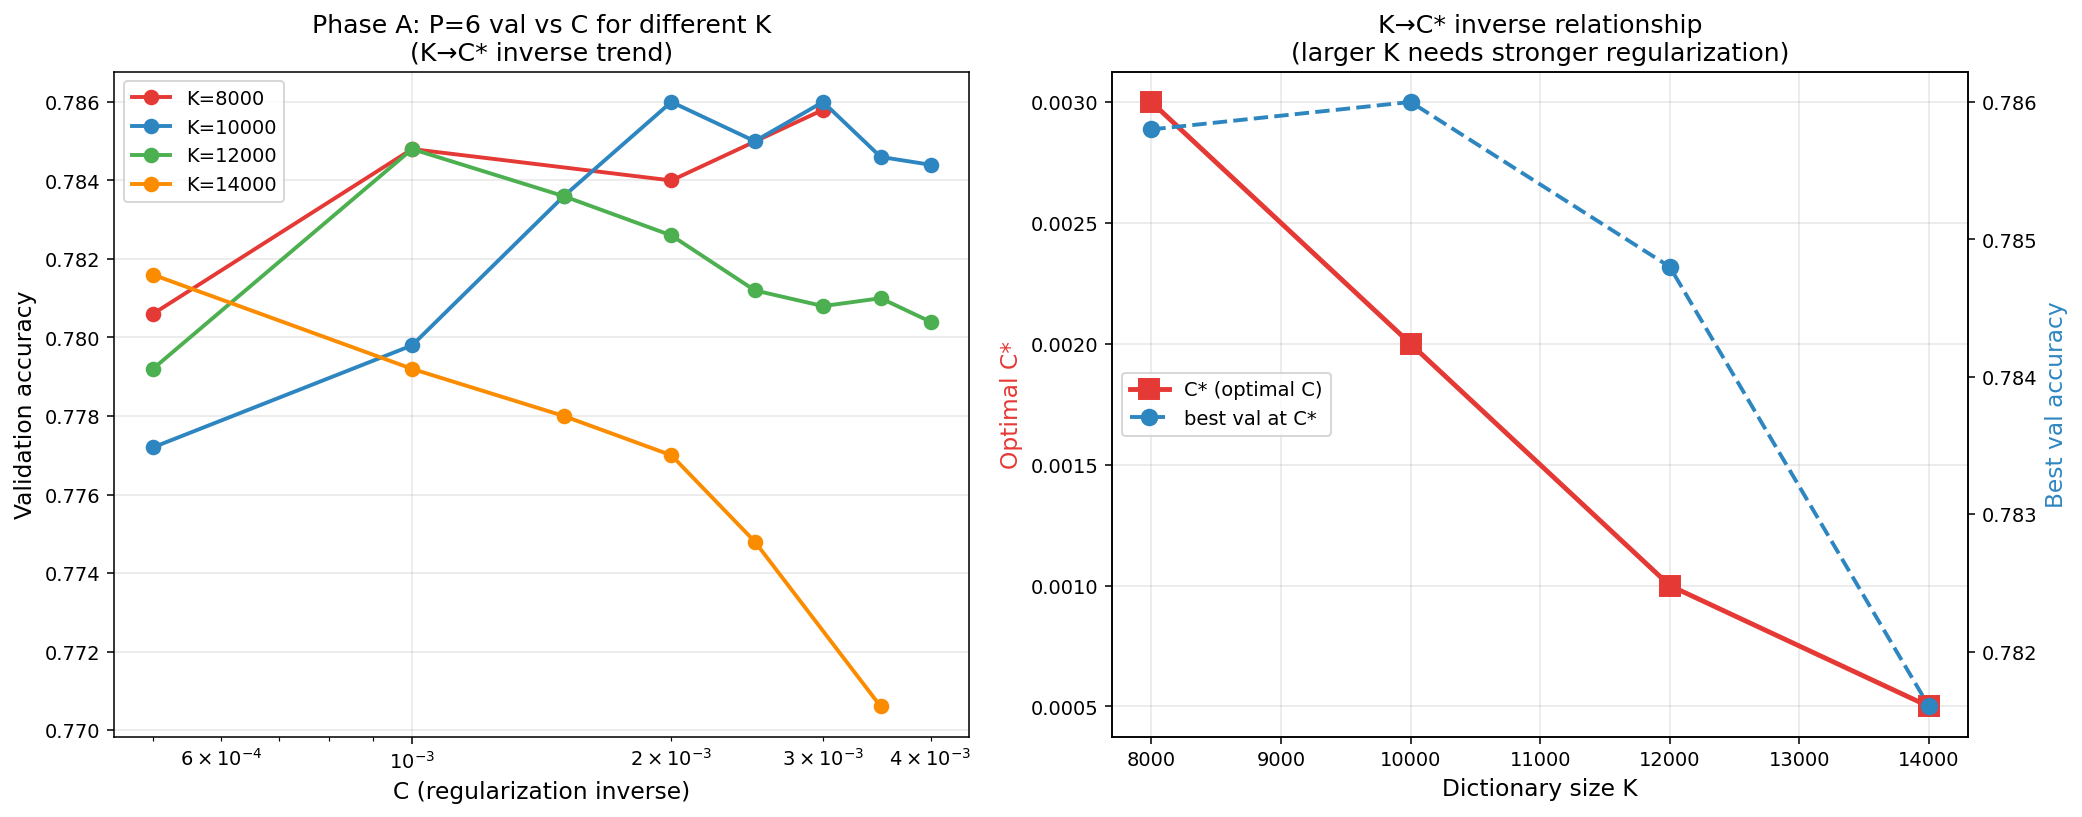
\includegraphics[width=0.75\linewidth]{figures/post07_02_phase_a_analysis.png}
  \caption{Phase A analysis: pushing dictionary size $K$ beyond 8000 for
  $P\!=\!6$.  Returns diminish rapidly past $K\!=\!10000$.}
  \label{fig:app_phase_a}
\end{figure}

\end{document}
